\section{core\_\-t Class Reference}
\label{classcore__t}\index{core\_\-t@{core\_\-t}}
{\tt \#include $<$zesto-core.h$>$}

Collaboration diagram for core\_\-t:\nopagebreak
\begin{figure}[H]
\begin{center}
\leavevmode
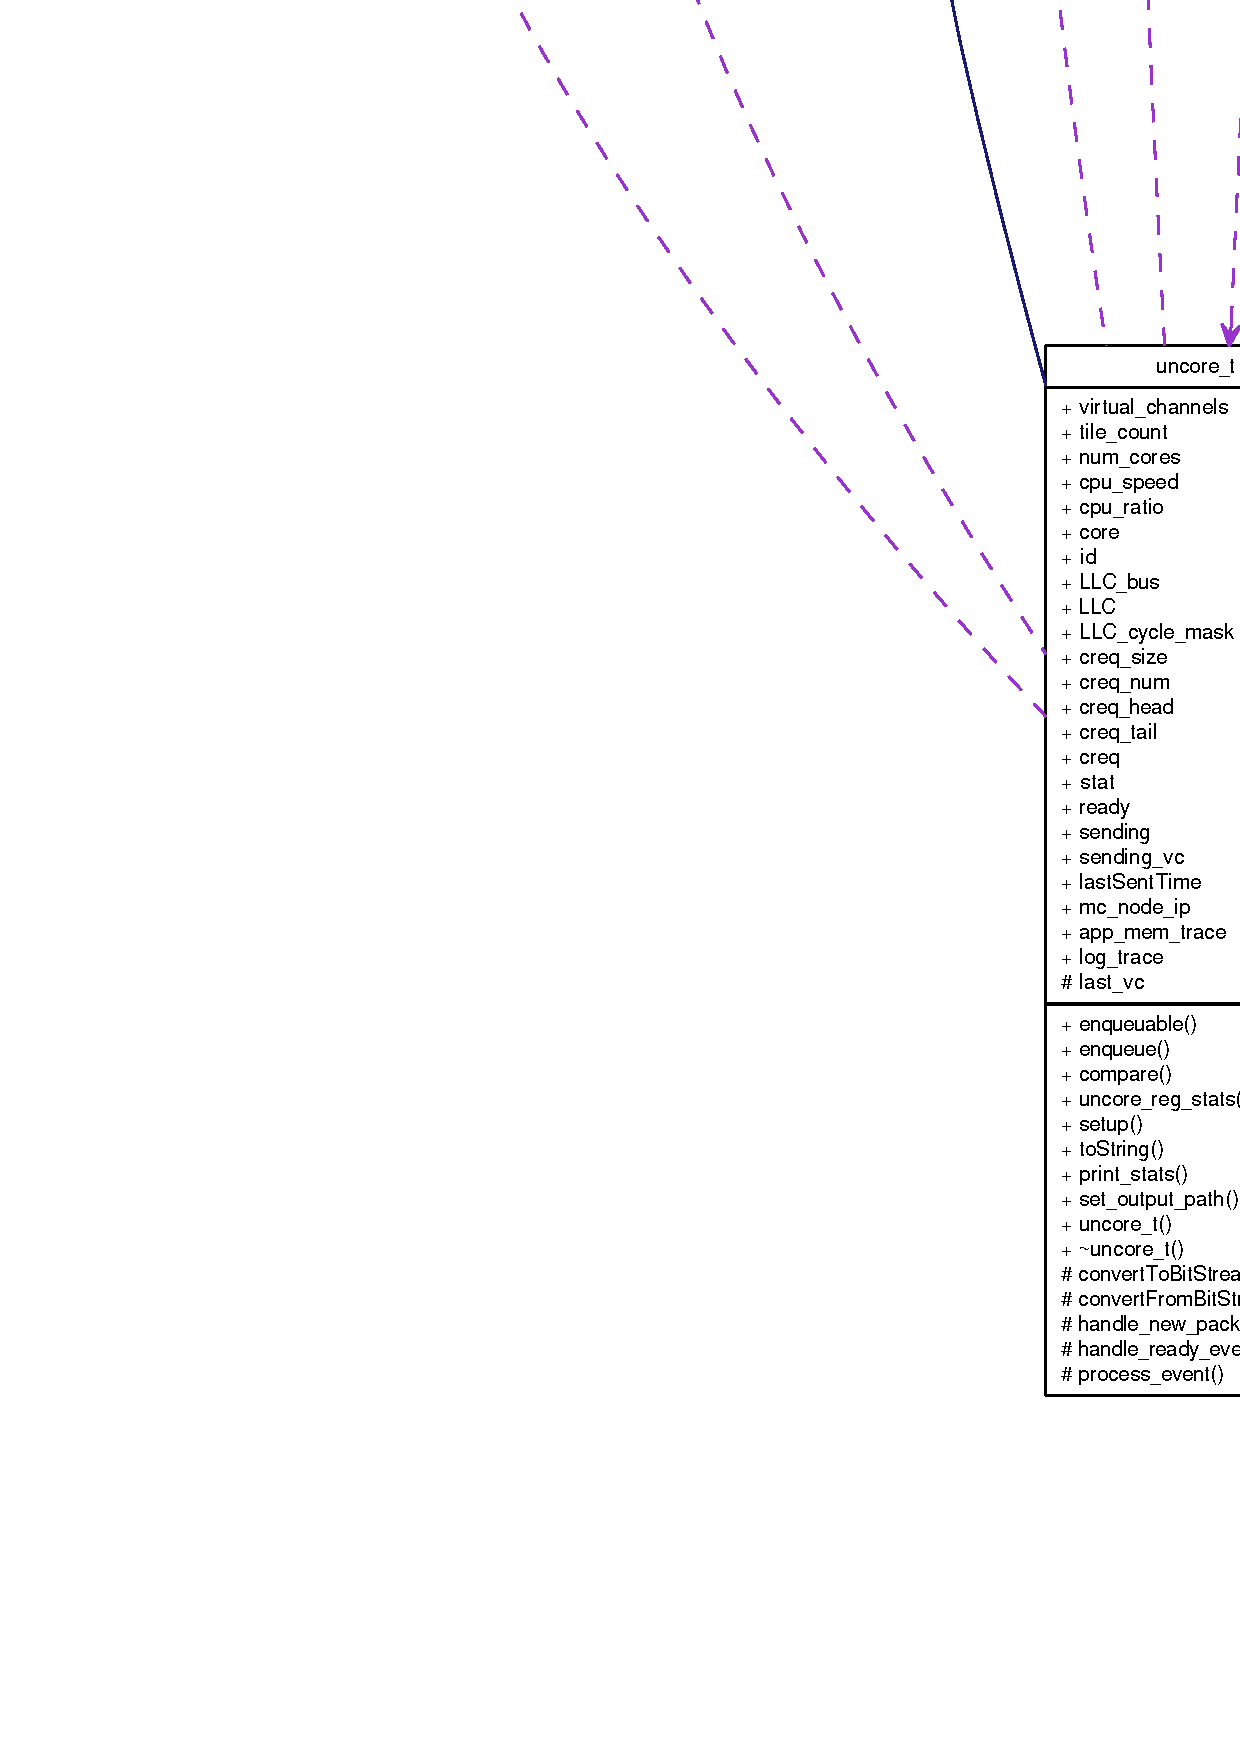
\includegraphics[width=400pt]{classcore__t__coll__graph}
\end{center}
\end{figure}
\subsection*{Classes}
\begin{CompactItemize}
\item 
struct {\bf core\_\-memory\_\-t}
\item 
struct {\bf core\_\-stat\_\-t}
\item 
struct {\bf uop\_\-array\_\-t}
\end{CompactItemize}
\subsection*{Public Member Functions}
\begin{CompactItemize}
\item 
{\bf core\_\-t} (const int core\_\-id)
\item 
{\bf seq\_\-t} {\bf new\_\-action\_\-id} (void)
\item 
struct {\bf uop\_\-t} $\ast$ {\bf get\_\-uop\_\-array} (const int size)
\item 
void {\bf return\_\-uop\_\-array} (struct {\bf uop\_\-t} $\ast$const p)
\item 
struct {\bf odep\_\-t} $\ast$ {\bf get\_\-odep\_\-link} (void)
\item 
void {\bf return\_\-odep\_\-link} (struct {\bf odep\_\-t} $\ast$const p)
\end{CompactItemize}
\subsection*{Static Public Member Functions}
\begin{CompactItemize}
\item 
static void {\bf zero\_\-uop} (struct {\bf uop\_\-t} $\ast$const uop)
\item 
static void {\bf zero\_\-Mop} (struct {\bf Mop\_\-t} $\ast$const Mop)
\end{CompactItemize}
\subsection*{Public Attributes}
\begin{CompactItemize}
\item 
struct {\bf core\_\-knobs\_\-t} $\ast$ {\bf knobs}
\item 
struct {\bf thread\_\-t} $\ast$ {\bf current\_\-thread}
\item 
int {\bf id}
\item 
struct {\bf uncore\_\-t} $\ast$ {\bf uncore}
\item 
{\bf counter\_\-t} {\bf num\_\-emergency\_\-recoveries}
\item 
int {\bf last\_\-emergency\_\-recovery\_\-count}
\item 
class {\bf core\_\-oracle\_\-t} $\ast$ {\bf oracle}
\item 
class {\bf core\_\-fetch\_\-t} $\ast$ {\bf fetch}
\item 
class {\bf core\_\-decode\_\-t} $\ast$ {\bf decode}
\item 
class {\bf core\_\-alloc\_\-t} $\ast$ {\bf alloc}
\item 
class {\bf core\_\-exec\_\-t} $\ast$ {\bf exec}
\item 
class {\bf core\_\-commit\_\-t} $\ast$ {\bf commit}
\item 
struct {\bf core\_\-t::core\_\-memory\_\-t} {\bf memory}
\item 
struct {\bf core\_\-t::core\_\-stat\_\-t} {\bf stat}
\end{CompactItemize}
\subsection*{Protected Member Functions}
\begin{CompactItemize}
\item 
void {\bf uop\_\-init} (struct {\bf uop\_\-t} $\ast$const uop)
\end{CompactItemize}
\subsection*{Protected Attributes}
\begin{CompactItemize}
\item 
{\bf seq\_\-t} {\bf global\_\-action\_\-id}
\end{CompactItemize}
\subsection*{Static Protected Attributes}
\begin{CompactItemize}
\item 
static bool {\bf static\_\-members\_\-initialized} = false
\item 
static {\bf seq\_\-t} {\bf global\_\-seq} = 0
\item 
static struct {\bf uop\_\-array\_\-t} $\ast$ {\bf uop\_\-array\_\-pool} [MD\_\-MAX\_\-FLOWLEN+2+1]
\item 
static struct {\bf odep\_\-t} $\ast$ {\bf odep\_\-free\_\-pool} = NULL
\item 
static int {\bf odep\_\-free\_\-pool\_\-debt} = 0
\end{CompactItemize}
\subsection*{Friends}
\begin{CompactItemize}
\item 
class {\bf core\_\-oracle\_\-t}
\end{CompactItemize}


\subsection{Detailed Description}


Definition at line 142 of file zesto-core.h.

\subsection{Constructor \& Destructor Documentation}
\index{core\_\-t@{core\_\-t}!core\_\-t@{core\_\-t}}
\index{core\_\-t@{core\_\-t}!core_t@{core\_\-t}}
\subsubsection[{core\_\-t}]{\setlength{\rightskip}{0pt plus 5cm}core\_\-t::core\_\-t (const int {\em core\_\-id})}\label{classcore__t_5bc9e3784ebc125c92ac3d84e0aed88a}




Definition at line 88 of file zesto-core.cpp.

References memory, memzero(), stat, static\_\-members\_\-initialized, and uop\_\-array\_\-pool.

Referenced by sim\_\-post\_\-init().

Here is the caller graph for this function:\nopagebreak
\begin{figure}[H]
\begin{center}
\leavevmode
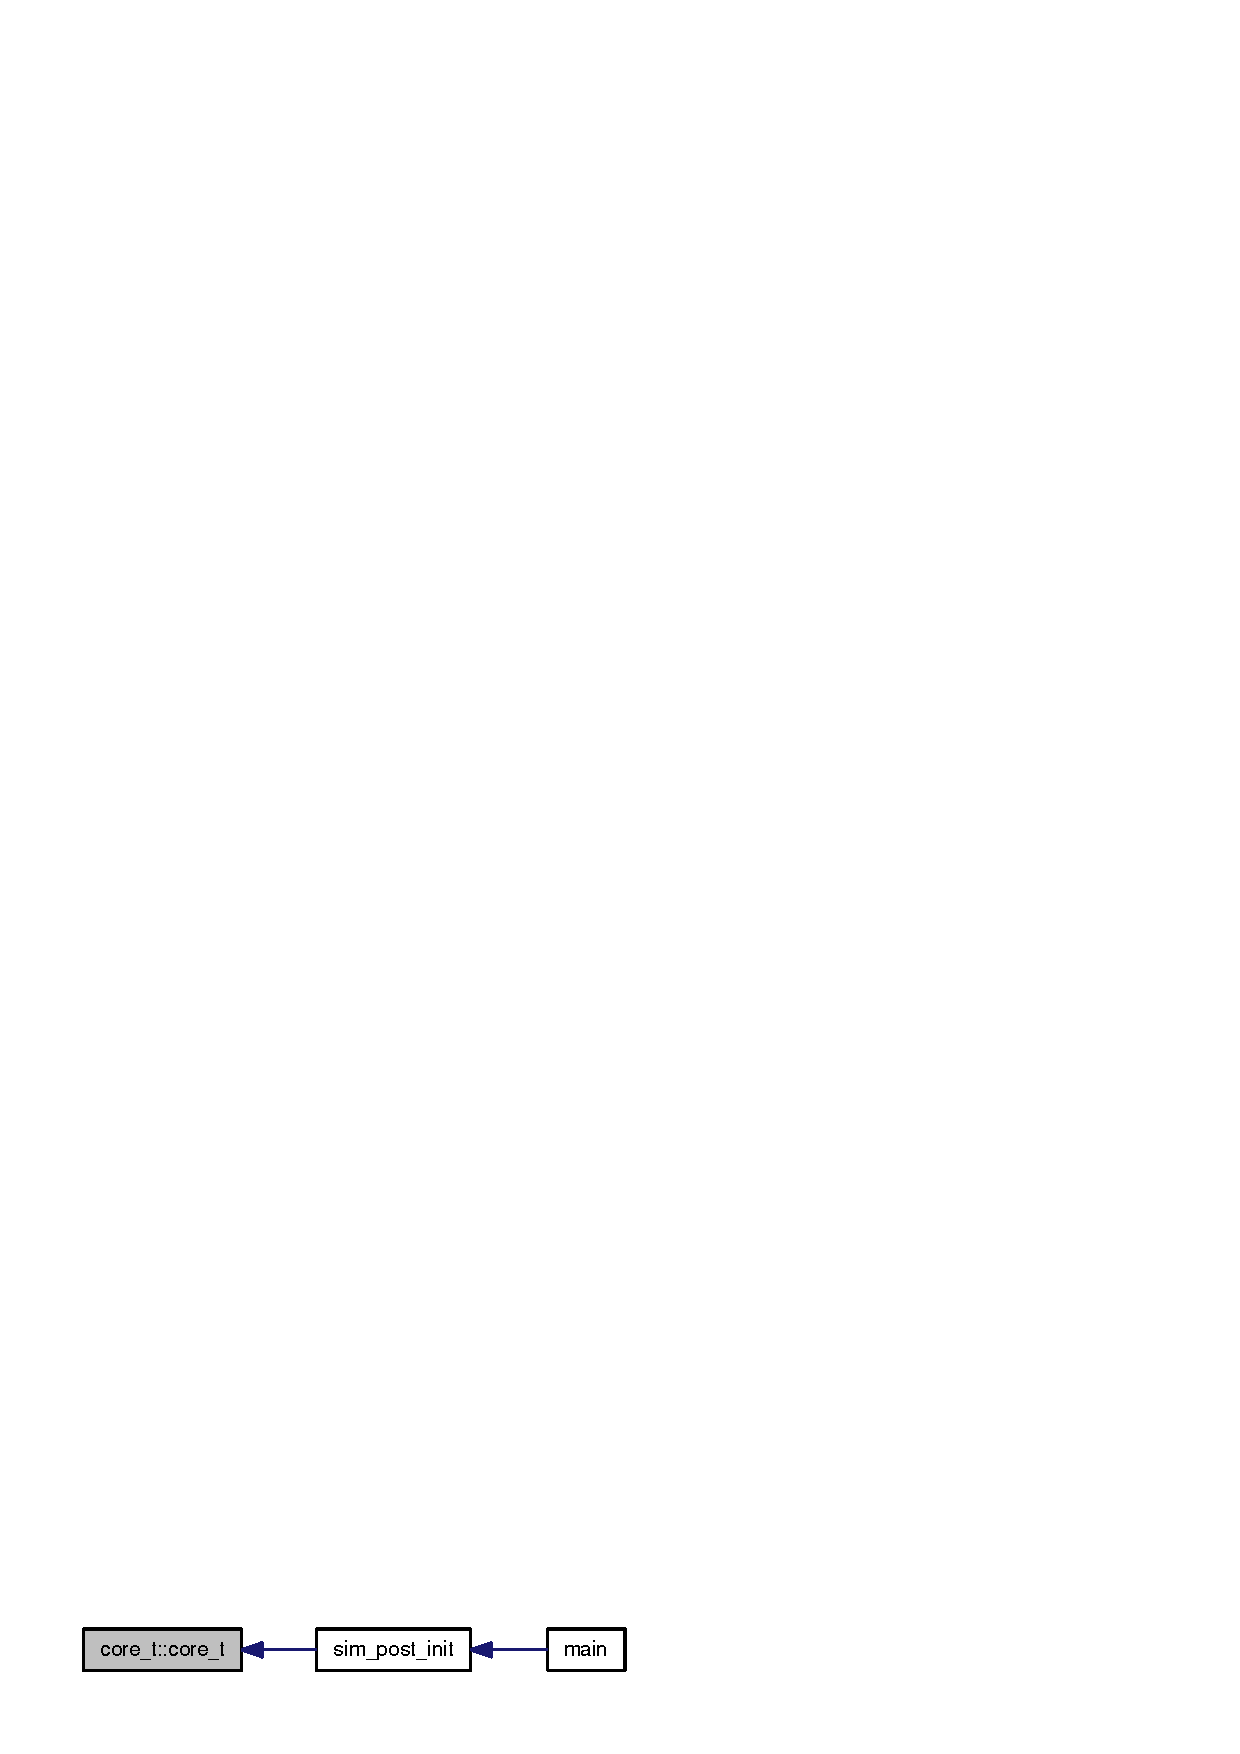
\includegraphics[width=152pt]{classcore__t_5bc9e3784ebc125c92ac3d84e0aed88a_icgraph}
\end{center}
\end{figure}


\subsection{Member Function Documentation}
\index{core\_\-t@{core\_\-t}!get\_\-odep\_\-link@{get\_\-odep\_\-link}}
\index{get\_\-odep\_\-link@{get\_\-odep\_\-link}!core_t@{core\_\-t}}
\subsubsection[{get\_\-odep\_\-link}]{\setlength{\rightskip}{0pt plus 5cm}struct {\bf odep\_\-t} $\ast$ core\_\-t::get\_\-odep\_\-link (void)\hspace{0.3cm}{\tt  [read]}}\label{classcore__t_c584461c992898648b8e0f8cf5931dfd}




Definition at line 162 of file zesto-core.cpp.

References fatal(), odep\_\-t::next, odep\_\-free\_\-pool, and odep\_\-free\_\-pool\_\-debt.

Referenced by core\_\-oracle\_\-t::install\_\-dependencies(), core\_\-alloc\_\-STM\_\-t::step(), and core\_\-alloc\_\-DPM\_\-t::step().

Here is the caller graph for this function:\nopagebreak
\begin{figure}[H]
\begin{center}
\leavevmode
\includegraphics[width=329pt]{classcore__t_c584461c992898648b8e0f8cf5931dfd_icgraph}
\end{center}
\end{figure}
\index{core\_\-t@{core\_\-t}!get\_\-uop\_\-array@{get\_\-uop\_\-array}}
\index{get\_\-uop\_\-array@{get\_\-uop\_\-array}!core_t@{core\_\-t}}
\subsubsection[{get\_\-uop\_\-array}]{\setlength{\rightskip}{0pt plus 5cm}struct {\bf uop\_\-t} $\ast$ core\_\-t::get\_\-uop\_\-array (const int {\em size})\hspace{0.3cm}{\tt  [read]}}\label{classcore__t_c7fc21b5fb694c21209262c29615fdb7}




Definition at line 123 of file zesto-core.cpp.

References fatal(), core\_\-t::core\_\-t::uop\_\-array\_\-t::next, core\_\-t::core\_\-t::uop\_\-array\_\-t::size, core\_\-t::core\_\-t::uop\_\-array\_\-t::uop, uop\_\-array\_\-pool, and uop\_\-init().

Referenced by core\_\-oracle\_\-t::exec(), core\_\-exec\_\-STM\_\-t::STQ\_\-deallocate\_\-std(), and core\_\-exec\_\-DPM\_\-t::STQ\_\-deallocate\_\-std().

Here is the caller graph for this function:\nopagebreak
\begin{figure}[H]
\begin{center}
\leavevmode
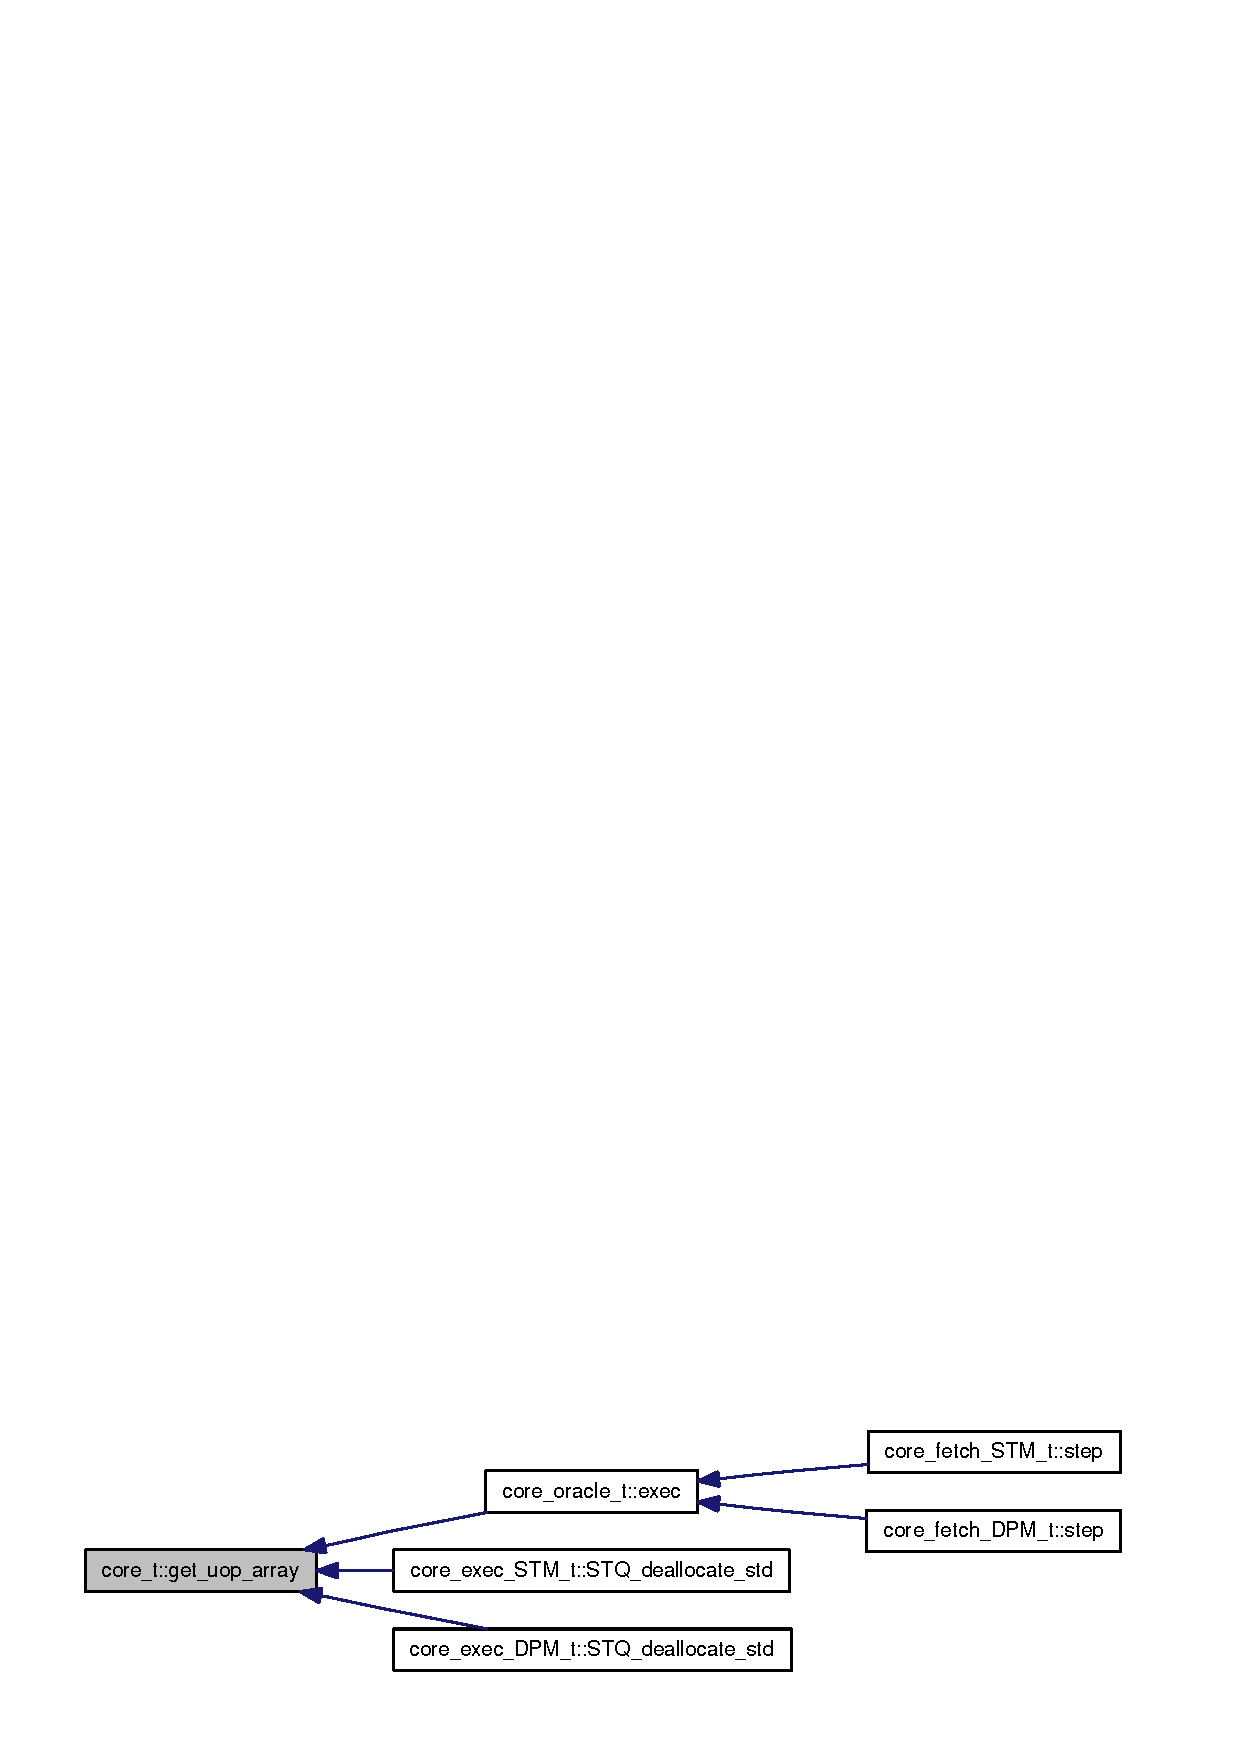
\includegraphics[width=271pt]{classcore__t_c7fc21b5fb694c21209262c29615fdb7_icgraph}
\end{center}
\end{figure}
\index{core\_\-t@{core\_\-t}!new\_\-action\_\-id@{new\_\-action\_\-id}}
\index{new\_\-action\_\-id@{new\_\-action\_\-id}!core_t@{core\_\-t}}
\subsubsection[{new\_\-action\_\-id}]{\setlength{\rightskip}{0pt plus 5cm}{\bf seq\_\-t} core\_\-t::new\_\-action\_\-id (void)}\label{classcore__t_110f33d959a11c403fb9166326c7e5f3}




Definition at line 107 of file zesto-core.cpp.

References global\_\-action\_\-id.

Referenced by core\_\-exec\_\-STM\_\-t::ALU\_\-exec(), core\_\-exec\_\-DPM\_\-t::ALU\_\-exec(), core\_\-fetch\_\-STM\_\-t::byteQ\_\-request(), core\_\-fetch\_\-DPM\_\-t::byteQ\_\-request(), core\_\-exec\_\-STM\_\-t::insert\_\-ready\_\-uop(), core\_\-exec\_\-DPM\_\-t::insert\_\-ready\_\-uop(), core\_\-fetch\_\-DPM\_\-t::jeclear\_\-enqueue(), core\_\-exec\_\-STM\_\-t::LDST\_\-exec(), core\_\-exec\_\-DPM\_\-t::LDST\_\-exec(), core\_\-fetch\_\-STM\_\-t::recover(), core\_\-fetch\_\-DPM\_\-t::recover(), core\_\-commit\_\-STM\_\-t::recover(), core\_\-commit\_\-DPM\_\-t::recover(), core\_\-exec\_\-DPM\_\-t::snatch\_\-back(), core\_\-commit\_\-STM\_\-t::step(), core\_\-commit\_\-DPM\_\-t::step(), core\_\-exec\_\-STM\_\-t::STQ\_\-deallocate\_\-std(), core\_\-exec\_\-DPM\_\-t::STQ\_\-deallocate\_\-std(), core\_\-exec\_\-DPM\_\-t::STQ\_\-squash\_\-senior(), core\_\-oracle\_\-t::undo(), and uop\_\-init().

Here is the caller graph for this function:\nopagebreak
\begin{figure}[H]
\begin{center}
\leavevmode
\includegraphics[width=420pt]{classcore__t_110f33d959a11c403fb9166326c7e5f3_icgraph}
\end{center}
\end{figure}
\index{core\_\-t@{core\_\-t}!return\_\-odep\_\-link@{return\_\-odep\_\-link}}
\index{return\_\-odep\_\-link@{return\_\-odep\_\-link}!core_t@{core\_\-t}}
\subsubsection[{return\_\-odep\_\-link}]{\setlength{\rightskip}{0pt plus 5cm}void core\_\-t::return\_\-odep\_\-link (struct {\bf odep\_\-t} $\ast$const  {\em p})}\label{classcore__t_c76899d81828f8557930f9ab87f4938e}




Definition at line 182 of file zesto-core.cpp.

References odep\_\-t::next, odep\_\-free\_\-pool, odep\_\-free\_\-pool\_\-debt, and odep\_\-t::uop.

Referenced by core\_\-oracle\_\-t::commit\_\-dependencies(), core\_\-oracle\_\-t::commit\_\-uop(), core\_\-commit\_\-STM\_\-t::recover(), core\_\-commit\_\-DPM\_\-t::recover(), and core\_\-oracle\_\-t::undo\_\-dependencies().

Here is the caller graph for this function:\nopagebreak
\begin{figure}[H]
\begin{center}
\leavevmode
\includegraphics[width=420pt]{classcore__t_c76899d81828f8557930f9ab87f4938e_icgraph}
\end{center}
\end{figure}
\index{core\_\-t@{core\_\-t}!return\_\-uop\_\-array@{return\_\-uop\_\-array}}
\index{return\_\-uop\_\-array@{return\_\-uop\_\-array}!core_t@{core\_\-t}}
\subsubsection[{return\_\-uop\_\-array}]{\setlength{\rightskip}{0pt plus 5cm}void core\_\-t::return\_\-uop\_\-array (struct {\bf uop\_\-t} $\ast$const  {\em p})}\label{classcore__t_466dcf5a0ecb9fd32ad557561286dfc9}




Definition at line 149 of file zesto-core.cpp.

References core\_\-t::core\_\-t::uop\_\-array\_\-t::next, core\_\-t::core\_\-t::uop\_\-array\_\-t::size, and uop\_\-array\_\-pool.

Referenced by core\_\-oracle\_\-t::exec(), core\_\-exec\_\-STM\_\-t::store\_\-dl1\_\-callback(), core\_\-exec\_\-DPM\_\-t::store\_\-dl1\_\-callback(), core\_\-exec\_\-DPM\_\-t::store\_\-dl1\_\-split\_\-callback(), core\_\-exec\_\-STM\_\-t::store\_\-dtlb\_\-callback(), and core\_\-exec\_\-DPM\_\-t::store\_\-dtlb\_\-callback().

Here is the caller graph for this function:\nopagebreak
\begin{figure}[H]
\begin{center}
\leavevmode
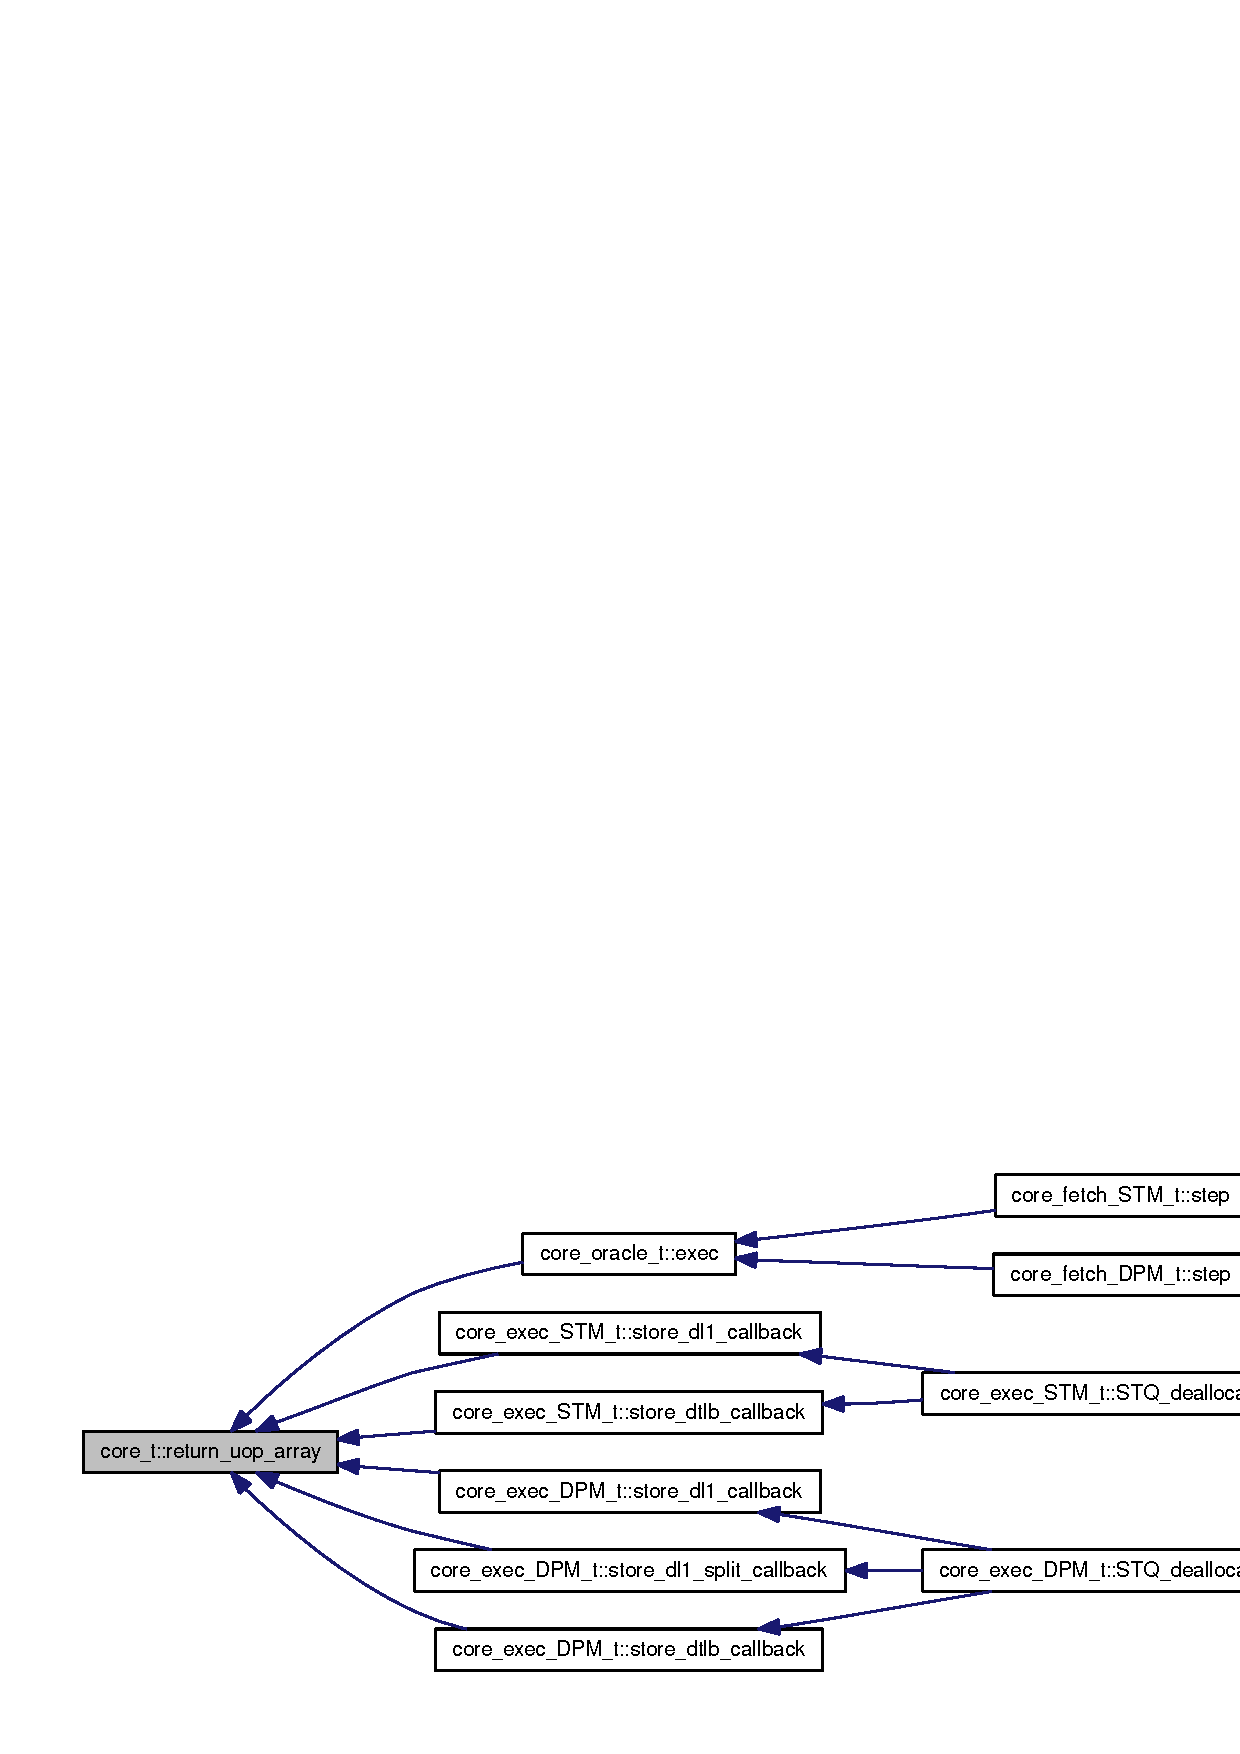
\includegraphics[width=319pt]{classcore__t_466dcf5a0ecb9fd32ad557561286dfc9_icgraph}
\end{center}
\end{figure}
\index{core\_\-t@{core\_\-t}!uop\_\-init@{uop\_\-init}}
\index{uop\_\-init@{uop\_\-init}!core_t@{core\_\-t}}
\subsubsection[{uop\_\-init}]{\setlength{\rightskip}{0pt plus 5cm}void core\_\-t::uop\_\-init (struct {\bf uop\_\-t} $\ast$const  {\em uop})\hspace{0.3cm}{\tt  [protected]}}\label{classcore__t_9e530ff1e928624b77e18ae6d99fbd28}




Definition at line 267 of file zesto-core.cpp.

References uop\_\-t::action\_\-id, uop\_\-t::alloc, uop\_\-t::core, uop\_\-t::decode, uop\_\-t::exec, MAX\_\-IDEPS, uop\_\-t::Mop\_\-seq, new\_\-action\_\-id(), uop\_\-t::port\_\-assignment, TICK\_\-T\_\-MAX, uop\_\-t::timing, uop\_\-t::uop\_\-seq, uop\_\-t::when\_\-addr\_\-translated, uop\_\-t::when\_\-allocated, uop\_\-t::when\_\-completed, uop\_\-t::when\_\-data\_\-loaded, uop\_\-t::when\_\-decoded, uop\_\-t::when\_\-exec, uop\_\-t::when\_\-issued, uop\_\-t::when\_\-itag\_\-ready, uop\_\-t::when\_\-ival\_\-ready, uop\_\-t::when\_\-otag\_\-ready, uop\_\-t::when\_\-ready, and zero\_\-uop().

Referenced by get\_\-uop\_\-array().

Here is the caller graph for this function:\nopagebreak
\begin{figure}[H]
\begin{center}
\leavevmode
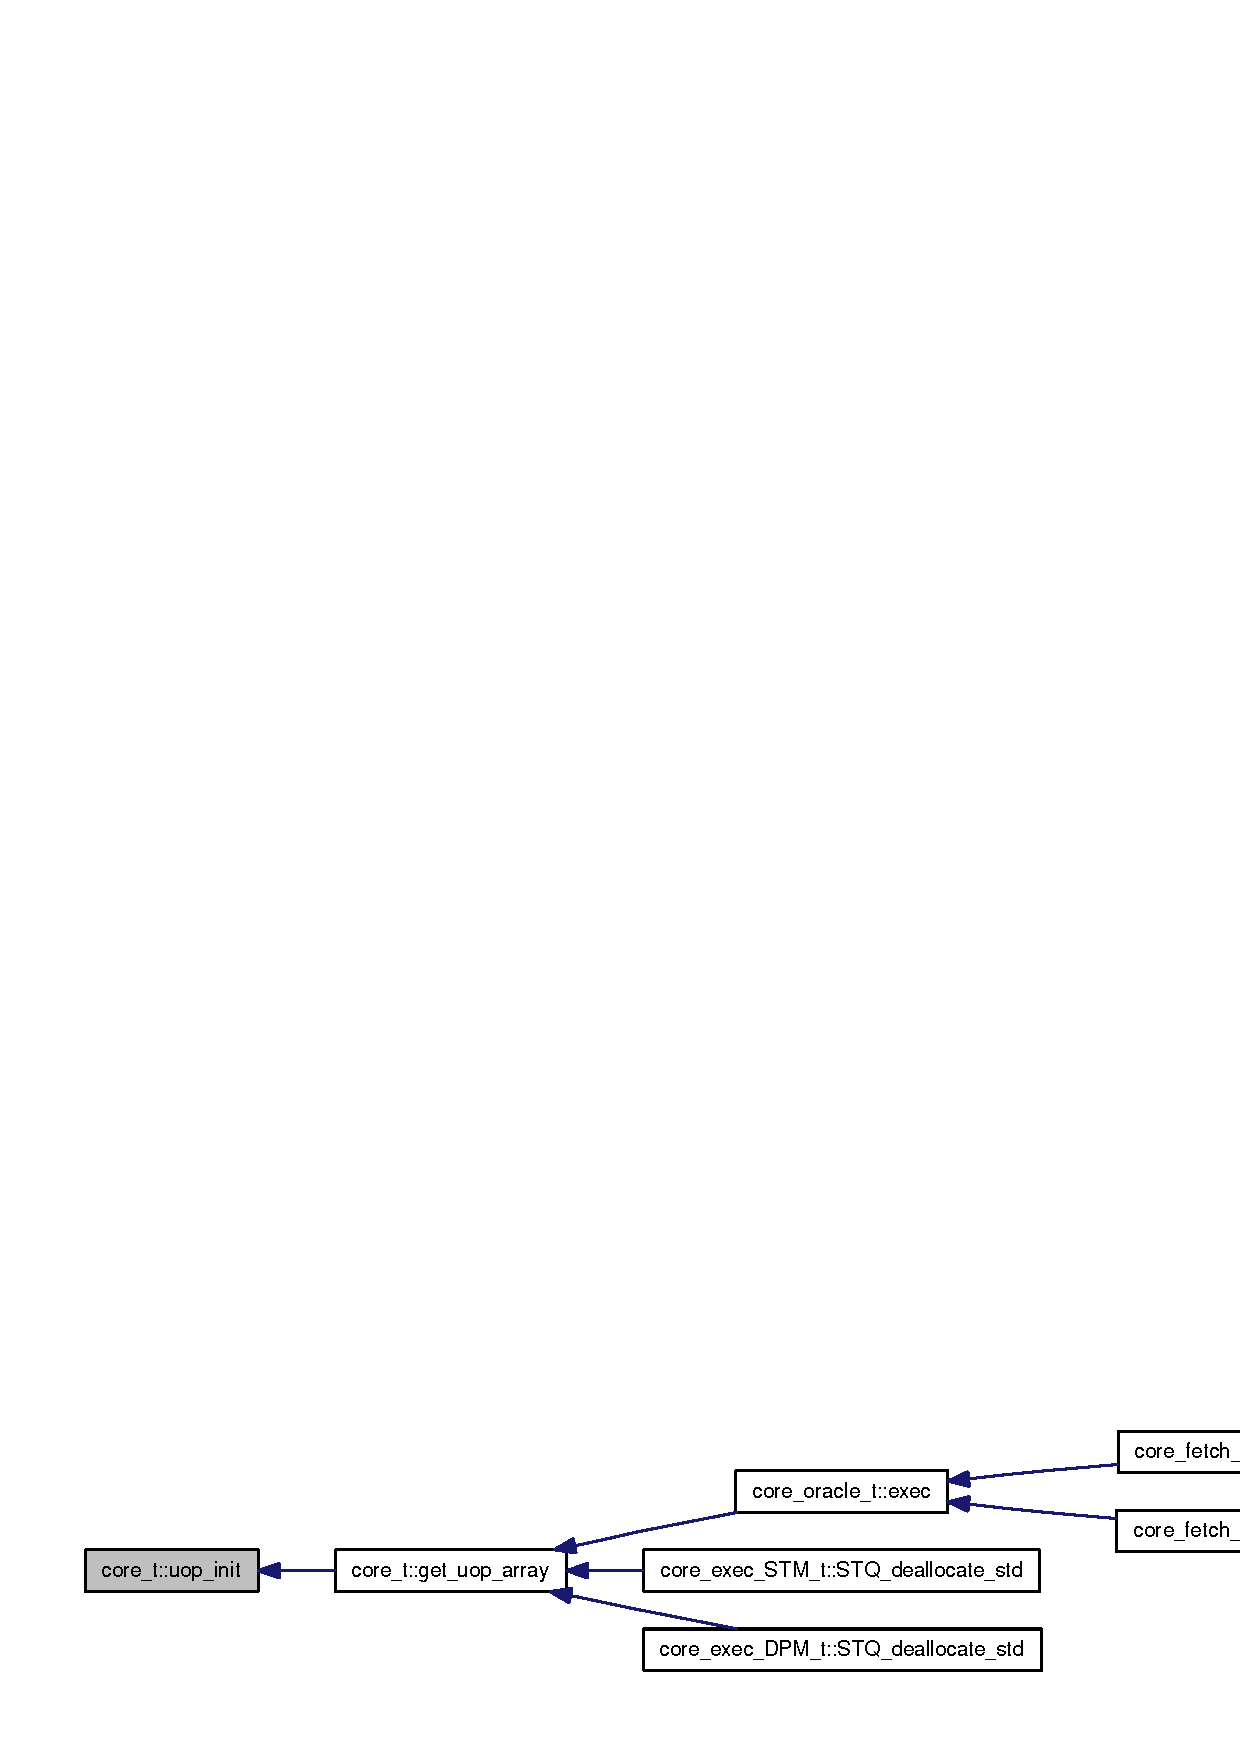
\includegraphics[width=331pt]{classcore__t_9e530ff1e928624b77e18ae6d99fbd28_icgraph}
\end{center}
\end{figure}
\index{core\_\-t@{core\_\-t}!zero\_\-Mop@{zero\_\-Mop}}
\index{zero\_\-Mop@{zero\_\-Mop}!core_t@{core\_\-t}}
\subsubsection[{zero\_\-Mop}]{\setlength{\rightskip}{0pt plus 5cm}void core\_\-t::zero\_\-Mop (struct {\bf Mop\_\-t} $\ast$const  {\em Mop})\hspace{0.3cm}{\tt  [static]}}\label{classcore__t_d9a45d86038d1410219106b4d6757052}




Definition at line 232 of file zesto-core.cpp.

Referenced by core\_\-oracle\_\-t::exec().

Here is the caller graph for this function:\nopagebreak
\begin{figure}[H]
\begin{center}
\leavevmode
\includegraphics[width=216pt]{classcore__t_d9a45d86038d1410219106b4d6757052_icgraph}
\end{center}
\end{figure}
\index{core\_\-t@{core\_\-t}!zero\_\-uop@{zero\_\-uop}}
\index{zero\_\-uop@{zero\_\-uop}!core_t@{core\_\-t}}
\subsubsection[{zero\_\-uop}]{\setlength{\rightskip}{0pt plus 5cm}void core\_\-t::zero\_\-uop (struct {\bf uop\_\-t} $\ast$const  {\em uop})\hspace{0.3cm}{\tt  [static]}}\label{classcore__t_bc4b88dc03f155338cac4dbc6a463be1}




Definition at line 194 of file zesto-core.cpp.

Referenced by uop\_\-init().

Here is the caller graph for this function:\nopagebreak
\begin{figure}[H]
\begin{center}
\leavevmode
\includegraphics[width=394pt]{classcore__t_bc4b88dc03f155338cac4dbc6a463be1_icgraph}
\end{center}
\end{figure}


\subsection{Friends And Related Function Documentation}
\index{core\_\-t@{core\_\-t}!core\_\-oracle\_\-t@{core\_\-oracle\_\-t}}
\index{core\_\-oracle\_\-t@{core\_\-oracle\_\-t}!core_t@{core\_\-t}}
\subsubsection[{core\_\-oracle\_\-t}]{\setlength{\rightskip}{0pt plus 5cm}friend class {\bf core\_\-oracle\_\-t}\hspace{0.3cm}{\tt  [friend]}}\label{classcore__t_28fd9847ad7d473828154837f3829666}




Definition at line 144 of file zesto-core.h.

\subsection{Member Data Documentation}
\index{core\_\-t@{core\_\-t}!alloc@{alloc}}
\index{alloc@{alloc}!core_t@{core\_\-t}}
\subsubsection[{alloc}]{\setlength{\rightskip}{0pt plus 5cm}class {\bf core\_\-alloc\_\-t}$\ast$ {\bf core\_\-t::alloc}}\label{classcore__t_20394b8c7a44d5ad56a16e9cd635299e}




Definition at line 195 of file zesto-core.h.

Referenced by core\_\-exec\_\-STM\_\-t::ALU\_\-exec(), core\_\-exec\_\-DPM\_\-t::ALU\_\-exec(), emergency\_\-recovery(), core\_\-oracle\_\-t::pipe\_\-recover(), core\_\-commit\_\-STM\_\-t::recover(), core\_\-commit\_\-DPM\_\-t::recover(), core\_\-oracle\_\-t::reset\_\-execution(), sim\_\-post\_\-init(), core\_\-fetch\_\-DPM\_\-t::step(), core\_\-commit\_\-STM\_\-t::step(), and core\_\-commit\_\-DPM\_\-t::step().\index{core\_\-t@{core\_\-t}!commit@{commit}}
\index{commit@{commit}!core_t@{core\_\-t}}
\subsubsection[{commit}]{\setlength{\rightskip}{0pt plus 5cm}class {\bf core\_\-commit\_\-t}$\ast$ {\bf core\_\-t::commit}}\label{classcore__t_1058815318dc1da3c60b90d9a5479092}




Definition at line 197 of file zesto-core.h.

Referenced by zesto\_\-component::downtick\_\-handler(), emergency\_\-recovery(), core\_\-oracle\_\-t::pipe\_\-recover(), core\_\-oracle\_\-t::reset\_\-execution(), sim\_\-post\_\-init(), core\_\-fetch\_\-DPM\_\-t::step(), core\_\-alloc\_\-STM\_\-t::step(), and core\_\-alloc\_\-DPM\_\-t::step().\index{core\_\-t@{core\_\-t}!current\_\-thread@{current\_\-thread}}
\index{current\_\-thread@{current\_\-thread}!core_t@{core\_\-t}}
\subsubsection[{current\_\-thread}]{\setlength{\rightskip}{0pt plus 5cm}struct {\bf thread\_\-t}$\ast$ {\bf core\_\-t::current\_\-thread}\hspace{0.3cm}{\tt  [read]}}\label{classcore__t_514a179d7ff004ee9a5c5167d90c2119}




Definition at line 179 of file zesto-core.h.

Referenced by bus\_\-reg\_\-stats(), cache\_\-reg\_\-stats(), core\_\-oracle\_\-t::complete\_\-flush(), emergency\_\-recovery(), core\_\-oracle\_\-t::exec(), core\_\-exec\_\-STM\_\-t::LDQ\_\-schedule(), core\_\-exec\_\-DPM\_\-t::LDQ\_\-schedule(), md\_\-fetch\_\-next\_\-pc(), core\_\-oracle\_\-t::pipe\_\-flush(), core\_\-oracle\_\-t::recover(), prefetch\_\-t::reg\_\-stats(), core\_\-oracle\_\-t::reg\_\-stats(), memdep\_\-t::reg\_\-stats(), bpred\_\-t::reg\_\-stats(), RAS\_\-t::reg\_\-stats(), BTB\_\-t::reg\_\-stats(), fusion\_\-t::reg\_\-stats(), bpred\_\-dir\_\-t::reg\_\-stats(), core\_\-fetch\_\-STM\_\-t::reg\_\-stats(), core\_\-fetch\_\-DPM\_\-t::reg\_\-stats(), core\_\-exec\_\-STM\_\-t::reg\_\-stats(), core\_\-exec\_\-DPM\_\-t::reg\_\-stats(), core\_\-decode\_\-STM\_\-t::reg\_\-stats(), core\_\-decode\_\-DPM\_\-t::reg\_\-stats(), core\_\-commit\_\-STM\_\-t::reg\_\-stats(), core\_\-commit\_\-DPM\_\-t::reg\_\-stats(), core\_\-alloc\_\-STM\_\-t::reg\_\-stats(), core\_\-alloc\_\-DPM\_\-t::reg\_\-stats(), core\_\-oracle\_\-t::reset\_\-execution(), sim\_\-fastfwd(), sim\_\-main(), sim\_\-post\_\-init(), core\_\-fetch\_\-STM\_\-t::step(), core\_\-fetch\_\-DPM\_\-t::step(), core\_\-commit\_\-STM\_\-t::step(), core\_\-commit\_\-DPM\_\-t::step(), core\_\-exec\_\-STM\_\-t::STQ\_\-deallocate\_\-std(), core\_\-exec\_\-DPM\_\-t::STQ\_\-deallocate\_\-std(), and core\_\-oracle\_\-t::undo().\index{core\_\-t@{core\_\-t}!decode@{decode}}
\index{decode@{decode}!core_t@{core\_\-t}}
\subsubsection[{decode}]{\setlength{\rightskip}{0pt plus 5cm}class {\bf core\_\-decode\_\-t}$\ast$ {\bf core\_\-t::decode}}\label{classcore__t_5a8f490b74ace2edeb7f90c493c98691}




Definition at line 194 of file zesto-core.h.

Referenced by zesto\_\-component::downtick\_\-handler(), emergency\_\-recovery(), core\_\-oracle\_\-t::pipe\_\-recover(), core\_\-oracle\_\-t::reset\_\-execution(), sim\_\-post\_\-init(), core\_\-fetch\_\-DPM\_\-t::step(), core\_\-commit\_\-STM\_\-t::step(), core\_\-commit\_\-DPM\_\-t::step(), core\_\-alloc\_\-STM\_\-t::step(), and core\_\-alloc\_\-DPM\_\-t::step().\index{core\_\-t@{core\_\-t}!exec@{exec}}
\index{exec@{exec}!core_t@{core\_\-t}}
\subsubsection[{exec}]{\setlength{\rightskip}{0pt plus 5cm}class {\bf core\_\-exec\_\-t}$\ast$ {\bf core\_\-t::exec}}\label{classcore__t_fd8831061ddb119a3abe035f7a482b55}




Definition at line 196 of file zesto-core.h.

Referenced by core\_\-exec\_\-STM\_\-t::ALU\_\-exec(), core\_\-exec\_\-STM\_\-t::DL1\_\-callback(), core\_\-exec\_\-DPM\_\-t::DL1\_\-callback(), core\_\-exec\_\-DPM\_\-t::DL1\_\-split\_\-callback(), zesto\_\-component::downtick\_\-handler(), core\_\-exec\_\-STM\_\-t::DTLB\_\-callback(), core\_\-exec\_\-DPM\_\-t::DTLB\_\-callback(), emergency\_\-recovery(), core\_\-exec\_\-DPM\_\-t::load\_\-miss\_\-reschedule(), core\_\-oracle\_\-t::pipe\_\-recover(), core\_\-commit\_\-STM\_\-t::recover(), core\_\-commit\_\-DPM\_\-t::recover(), core\_\-oracle\_\-t::reset\_\-execution(), sim\_\-post\_\-init(), core\_\-fetch\_\-DPM\_\-t::step(), core\_\-commit\_\-STM\_\-t::step(), core\_\-commit\_\-DPM\_\-t::step(), core\_\-alloc\_\-STM\_\-t::step(), core\_\-alloc\_\-DPM\_\-t::step(), core\_\-exec\_\-DPM\_\-t::store\_\-dl1\_\-callback(), core\_\-exec\_\-DPM\_\-t::store\_\-dl1\_\-split\_\-callback(), core\_\-exec\_\-DPM\_\-t::store\_\-dtlb\_\-callback(), and core\_\-exec\_\-DPM\_\-t::store\_\-translated\_\-callback().\index{core\_\-t@{core\_\-t}!fetch@{fetch}}
\index{fetch@{fetch}!core_t@{core\_\-t}}
\subsubsection[{fetch}]{\setlength{\rightskip}{0pt plus 5cm}class {\bf core\_\-fetch\_\-t}$\ast$ {\bf core\_\-t::fetch}}\label{classcore__t_bb3b5f18fa768382f617bcdec3ee7d7e}




Definition at line 193 of file zesto-core.h.

Referenced by core\_\-decode\_\-STM\_\-t::check\_\-target(), core\_\-decode\_\-DPM\_\-t::check\_\-target(), core\_\-oracle\_\-t::complete\_\-flush(), zesto\_\-component::downtick\_\-handler(), emergency\_\-recovery(), core\_\-oracle\_\-t::exec(), md\_\-fetch\_\-next\_\-pc(), core\_\-oracle\_\-t::pipe\_\-recover(), core\_\-oracle\_\-t::recover(), core\_\-oracle\_\-t::reset\_\-execution(), sim\_\-fastfwd(), sim\_\-main(), sim\_\-post\_\-init(), core\_\-decode\_\-STM\_\-t::step(), core\_\-decode\_\-DPM\_\-t::step(), core\_\-commit\_\-STM\_\-t::step(), and core\_\-commit\_\-DPM\_\-t::step().\index{core\_\-t@{core\_\-t}!global\_\-action\_\-id@{global\_\-action\_\-id}}
\index{global\_\-action\_\-id@{global\_\-action\_\-id}!core_t@{core\_\-t}}
\subsubsection[{global\_\-action\_\-id}]{\setlength{\rightskip}{0pt plus 5cm}{\bf seq\_\-t} {\bf core\_\-t::global\_\-action\_\-id}\hspace{0.3cm}{\tt  [protected]}}\label{classcore__t_1831df5e3a0845e40a38f47b044b4d05}




Definition at line 360 of file zesto-core.h.

Referenced by new\_\-action\_\-id().\index{core\_\-t@{core\_\-t}!global\_\-seq@{global\_\-seq}}
\index{global\_\-seq@{global\_\-seq}!core_t@{core\_\-t}}
\subsubsection[{global\_\-seq}]{\setlength{\rightskip}{0pt plus 5cm}{\bf seq\_\-t} {\bf core\_\-t::global\_\-seq} = 0\hspace{0.3cm}{\tt  [static, protected]}}\label{classcore__t_d4bb322114e12a61f9c86ab9e30cb78a}




Definition at line 363 of file zesto-core.h.

Referenced by core\_\-oracle\_\-t::exec().\index{core\_\-t@{core\_\-t}!id@{id}}
\index{id@{id}!core_t@{core\_\-t}}
\subsubsection[{id}]{\setlength{\rightskip}{0pt plus 5cm}int {\bf core\_\-t::id}}\label{classcore__t_3a8653bac0ed9aefff8d1679ca81546f}




Definition at line 180 of file zesto-core.h.

Referenced by emergency\_\-recovery(), core\_\-oracle\_\-t::exec(), LLC\_\-reg\_\-stats(), core\_\-oracle\_\-t::pipe\_\-flush(), and sim\_\-fastfwd().\index{core\_\-t@{core\_\-t}!knobs@{knobs}}
\index{knobs@{knobs}!core_t@{core\_\-t}}
\subsubsection[{knobs}]{\setlength{\rightskip}{0pt plus 5cm}struct {\bf core\_\-knobs\_\-t}$\ast$ {\bf core\_\-t::knobs}\hspace{0.3cm}{\tt  [read]}}\label{classcore__t_a397a3f36f045e3c2a19dafc16dab1c1}




Definition at line 174 of file zesto-core.h.

Referenced by core\_\-exec\_\-STM\_\-t::ALU\_\-exec(), core\_\-exec\_\-DPM\_\-t::ALU\_\-exec(), core\_\-fetch\_\-STM\_\-t::byteQ\_\-already\_\-requested(), core\_\-fetch\_\-DPM\_\-t::byteQ\_\-already\_\-requested(), core\_\-fetch\_\-STM\_\-t::byteQ\_\-is\_\-full(), core\_\-fetch\_\-DPM\_\-t::byteQ\_\-is\_\-full(), core\_\-fetch\_\-STM\_\-t::byteQ\_\-request(), core\_\-fetch\_\-DPM\_\-t::byteQ\_\-request(), core\_\-decode\_\-STM\_\-t::check\_\-flush(), core\_\-decode\_\-DPM\_\-t::check\_\-flush(), core\_\-exec\_\-STM\_\-t::check\_\-load\_\-issue\_\-conditions(), core\_\-exec\_\-DPM\_\-t::check\_\-load\_\-issue\_\-conditions(), core\_\-alloc\_\-DPM\_\-t::core\_\-alloc\_\-DPM\_\-t(), core\_\-alloc\_\-STM\_\-t::core\_\-alloc\_\-STM\_\-t(), core\_\-commit\_\-DPM\_\-t::core\_\-commit\_\-DPM\_\-t(), core\_\-commit\_\-STM\_\-t::core\_\-commit\_\-STM\_\-t(), core\_\-decode\_\-DPM\_\-t::core\_\-decode\_\-DPM\_\-t(), core\_\-decode\_\-STM\_\-t::core\_\-decode\_\-STM\_\-t(), core\_\-exec\_\-DPM\_\-t::core\_\-exec\_\-DPM\_\-t(), core\_\-exec\_\-STM\_\-t::core\_\-exec\_\-STM\_\-t(), core\_\-fetch\_\-DPM\_\-t::core\_\-fetch\_\-DPM\_\-t(), core\_\-fetch\_\-STM\_\-t::core\_\-fetch\_\-STM\_\-t(), core\_\-oracle\_\-t::core\_\-oracle\_\-t(), core\_\-oracle\_\-t::exec(), core\_\-exec\_\-STM\_\-t::insert\_\-ready\_\-uop(), core\_\-exec\_\-DPM\_\-t::insert\_\-ready\_\-uop(), core\_\-exec\_\-STM\_\-t::LDQ\_\-available(), core\_\-exec\_\-DPM\_\-t::LDQ\_\-available(), core\_\-exec\_\-STM\_\-t::LDQ\_\-deallocate(), core\_\-exec\_\-DPM\_\-t::LDQ\_\-deallocate(), core\_\-exec\_\-STM\_\-t::LDQ\_\-insert(), core\_\-exec\_\-DPM\_\-t::LDQ\_\-insert(), core\_\-exec\_\-STM\_\-t::LDQ\_\-schedule(), core\_\-exec\_\-DPM\_\-t::LDQ\_\-schedule(), core\_\-exec\_\-STM\_\-t::LDQ\_\-squash(), core\_\-exec\_\-DPM\_\-t::LDQ\_\-squash(), core\_\-exec\_\-STM\_\-t::LDST\_\-exec(), core\_\-exec\_\-DPM\_\-t::LDST\_\-exec(), core\_\-exec\_\-DPM\_\-t::load\_\-miss\_\-reschedule(), core\_\-exec\_\-STM\_\-t::load\_\-writeback(), core\_\-exec\_\-DPM\_\-t::load\_\-writeback(), core\_\-fetch\_\-STM\_\-t::Mop\_\-consume(), core\_\-fetch\_\-DPM\_\-t::Mop\_\-consume(), core\_\-oracle\_\-t::pipe\_\-recover(), core\_\-fetch\_\-DPM\_\-t::predecode\_\-enqueue(), core\_\-fetch\_\-STM\_\-t::recover(), core\_\-fetch\_\-DPM\_\-t::recover(), core\_\-decode\_\-STM\_\-t::recover(), core\_\-decode\_\-DPM\_\-t::recover(), core\_\-commit\_\-STM\_\-t::recover(), core\_\-commit\_\-DPM\_\-t::recover(), core\_\-alloc\_\-DPM\_\-t::recover(), core\_\-decode\_\-DPM\_\-t::recover\_\-decode\_\-pipe(), core\_\-decode\_\-DPM\_\-t::recover\_\-uopQ(), core\_\-commit\_\-STM\_\-t::ROB\_\-available(), core\_\-commit\_\-DPM\_\-t::ROB\_\-available(), core\_\-commit\_\-STM\_\-t::ROB\_\-insert(), core\_\-commit\_\-DPM\_\-t::ROB\_\-insert(), core\_\-exec\_\-STM\_\-t::RS\_\-available(), core\_\-exec\_\-DPM\_\-t::RS\_\-available(), core\_\-exec\_\-STM\_\-t::RS\_\-deallocate(), core\_\-exec\_\-DPM\_\-t::RS\_\-deallocate(), core\_\-exec\_\-STM\_\-t::RS\_\-insert(), core\_\-exec\_\-DPM\_\-t::RS\_\-insert(), core\_\-exec\_\-STM\_\-t::RS\_\-schedule(), core\_\-exec\_\-DPM\_\-t::RS\_\-schedule(), sim\_\-post\_\-init(), core\_\-exec\_\-DPM\_\-t::snatch\_\-back(), core\_\-fetch\_\-STM\_\-t::step(), core\_\-fetch\_\-DPM\_\-t::step(), core\_\-decode\_\-STM\_\-t::step(), core\_\-decode\_\-DPM\_\-t::step(), core\_\-commit\_\-STM\_\-t::step(), core\_\-commit\_\-DPM\_\-t::step(), core\_\-alloc\_\-STM\_\-t::step(), core\_\-alloc\_\-DPM\_\-t::step(), core\_\-exec\_\-STM\_\-t::store\_\-dl1\_\-callback(), core\_\-exec\_\-DPM\_\-t::store\_\-dl1\_\-callback(), core\_\-exec\_\-DPM\_\-t::store\_\-dl1\_\-split\_\-callback(), core\_\-exec\_\-STM\_\-t::store\_\-dtlb\_\-callback(), core\_\-exec\_\-DPM\_\-t::store\_\-dtlb\_\-callback(), core\_\-exec\_\-DPM\_\-t::store\_\-translated\_\-callback(), core\_\-exec\_\-STM\_\-t::STQ\_\-available(), core\_\-exec\_\-DPM\_\-t::STQ\_\-available(), core\_\-exec\_\-DPM\_\-t::STQ\_\-deallocate\_\-senior(), core\_\-exec\_\-STM\_\-t::STQ\_\-deallocate\_\-std(), core\_\-exec\_\-DPM\_\-t::STQ\_\-deallocate\_\-std(), core\_\-exec\_\-STM\_\-t::STQ\_\-insert\_\-sta(), core\_\-exec\_\-DPM\_\-t::STQ\_\-insert\_\-sta(), core\_\-exec\_\-STM\_\-t::STQ\_\-insert\_\-std(), core\_\-exec\_\-DPM\_\-t::STQ\_\-insert\_\-std(), core\_\-exec\_\-DPM\_\-t::STQ\_\-squash\_\-senior(), core\_\-exec\_\-STM\_\-t::STQ\_\-squash\_\-sta(), core\_\-exec\_\-DPM\_\-t::STQ\_\-squash\_\-sta(), core\_\-exec\_\-STM\_\-t::STQ\_\-squash\_\-std(), core\_\-exec\_\-DPM\_\-t::STQ\_\-squash\_\-std(), core\_\-oracle\_\-t::syscall\_\-mem\_\-access(), core\_\-decode\_\-STM\_\-t::uop\_\-available(), core\_\-decode\_\-STM\_\-t::uop\_\-consume(), core\_\-decode\_\-DPM\_\-t::uop\_\-consume(), core\_\-decode\_\-STM\_\-t::uop\_\-peek(), core\_\-fetch\_\-DPM\_\-t::update\_\-occupancy(), core\_\-exec\_\-STM\_\-t::update\_\-occupancy(), core\_\-exec\_\-DPM\_\-t::update\_\-occupancy(), core\_\-decode\_\-DPM\_\-t::update\_\-occupancy(), core\_\-commit\_\-STM\_\-t::update\_\-occupancy(), and core\_\-commit\_\-DPM\_\-t::update\_\-occupancy().\index{core\_\-t@{core\_\-t}!last\_\-emergency\_\-recovery\_\-count@{last\_\-emergency\_\-recovery\_\-count}}
\index{last\_\-emergency\_\-recovery\_\-count@{last\_\-emergency\_\-recovery\_\-count}!core_t@{core\_\-t}}
\subsubsection[{last\_\-emergency\_\-recovery\_\-count}]{\setlength{\rightskip}{0pt plus 5cm}int {\bf core\_\-t::last\_\-emergency\_\-recovery\_\-count}}\label{classcore__t_11034d8bb95a7d541a7a0d5efdaded9a}




Definition at line 186 of file zesto-core.h.

Referenced by emergency\_\-recovery().\index{core\_\-t@{core\_\-t}!memory@{memory}}
\index{memory@{memory}!core_t@{core\_\-t}}
\subsubsection[{memory}]{\setlength{\rightskip}{0pt plus 5cm}struct {\bf core\_\-t::core\_\-memory\_\-t}  {\bf core\_\-t::memory}}\label{classcore__t_05317565ca33e18c2eb9b8fa9a950ce1}




Referenced by cache\_\-freeze\_\-stats(), cache\_\-process(), core\_\-exec\_\-DPM\_\-t::core\_\-exec\_\-DPM\_\-t(), core\_\-exec\_\-STM\_\-t::core\_\-exec\_\-STM\_\-t(), core\_\-fetch\_\-DPM\_\-t::core\_\-fetch\_\-DPM\_\-t(), core\_\-fetch\_\-STM\_\-t::core\_\-fetch\_\-STM\_\-t(), core\_\-t(), emergency\_\-recovery(), core\_\-exec\_\-STM\_\-t::LDQ\_\-schedule(), core\_\-exec\_\-DPM\_\-t::LDQ\_\-schedule(), core\_\-exec\_\-STM\_\-t::LDST\_\-exec(), core\_\-exec\_\-DPM\_\-t::LDST\_\-exec(), prefetch\_\-core\_\-caches(), core\_\-fetch\_\-STM\_\-t::reg\_\-stats(), core\_\-fetch\_\-DPM\_\-t::reg\_\-stats(), core\_\-exec\_\-STM\_\-t::reg\_\-stats(), core\_\-exec\_\-DPM\_\-t::reg\_\-stats(), core\_\-exec\_\-DPM\_\-t::RS\_\-schedule(), sim\_\-fastfwd(), core\_\-fetch\_\-STM\_\-t::step(), core\_\-fetch\_\-DPM\_\-t::step(), step\_\-core\_\-PF\_\-controllers(), core\_\-exec\_\-STM\_\-t::STQ\_\-deallocate\_\-std(), and core\_\-exec\_\-DPM\_\-t::STQ\_\-deallocate\_\-std().\index{core\_\-t@{core\_\-t}!num\_\-emergency\_\-recoveries@{num\_\-emergency\_\-recoveries}}
\index{num\_\-emergency\_\-recoveries@{num\_\-emergency\_\-recoveries}!core_t@{core\_\-t}}
\subsubsection[{num\_\-emergency\_\-recoveries}]{\setlength{\rightskip}{0pt plus 5cm}{\bf counter\_\-t} {\bf core\_\-t::num\_\-emergency\_\-recoveries}}\label{classcore__t_ad184ce68308f37e1fb07a5eab624314}




Definition at line 185 of file zesto-core.h.

Referenced by emergency\_\-recovery(), and core\_\-oracle\_\-t::reg\_\-stats().\index{core\_\-t@{core\_\-t}!odep\_\-free\_\-pool@{odep\_\-free\_\-pool}}
\index{odep\_\-free\_\-pool@{odep\_\-free\_\-pool}!core_t@{core\_\-t}}
\subsubsection[{odep\_\-free\_\-pool}]{\setlength{\rightskip}{0pt plus 5cm}struct {\bf odep\_\-t} $\ast$ {\bf core\_\-t::odep\_\-free\_\-pool} = NULL\hspace{0.3cm}{\tt  [static, read, protected]}}\label{classcore__t_3661ae39476a6b7fd401555ed7cdca6a}




Definition at line 368 of file zesto-core.h.

Referenced by get\_\-odep\_\-link(), and return\_\-odep\_\-link().\index{core\_\-t@{core\_\-t}!odep\_\-free\_\-pool\_\-debt@{odep\_\-free\_\-pool\_\-debt}}
\index{odep\_\-free\_\-pool\_\-debt@{odep\_\-free\_\-pool\_\-debt}!core_t@{core\_\-t}}
\subsubsection[{odep\_\-free\_\-pool\_\-debt}]{\setlength{\rightskip}{0pt plus 5cm}int {\bf core\_\-t::odep\_\-free\_\-pool\_\-debt} = 0\hspace{0.3cm}{\tt  [static, protected]}}\label{classcore__t_481bb5edace5509f6a976456c1e6b277}




Definition at line 369 of file zesto-core.h.

Referenced by get\_\-odep\_\-link(), and return\_\-odep\_\-link().\index{core\_\-t@{core\_\-t}!oracle@{oracle}}
\index{oracle@{oracle}!core_t@{core\_\-t}}
\subsubsection[{oracle}]{\setlength{\rightskip}{0pt plus 5cm}class {\bf core\_\-oracle\_\-t}$\ast$ {\bf core\_\-t::oracle}}\label{classcore__t_e4ae7e910eea6077916a780537d3210e}




Definition at line 192 of file zesto-core.h.

Referenced by core\_\-exec\_\-STM\_\-t::ALU\_\-exec(), core\_\-exec\_\-DPM\_\-t::ALU\_\-exec(), core\_\-decode\_\-STM\_\-t::check\_\-target(), core\_\-decode\_\-DPM\_\-t::check\_\-target(), zesto\_\-component::downtick\_\-handler(), emergency\_\-recovery(), core\_\-exec\_\-DPM\_\-t::LDQ\_\-schedule(), core\_\-exec\_\-STM\_\-t::LDST\_\-exec(), core\_\-exec\_\-DPM\_\-t::LDST\_\-exec(), core\_\-exec\_\-STM\_\-t::load\_\-writeback(), core\_\-exec\_\-DPM\_\-t::load\_\-writeback(), core\_\-fetch\_\-STM\_\-t::Mop\_\-consume(), core\_\-fetch\_\-STM\_\-t::Mop\_\-peek(), sim\_\-post\_\-init(), core\_\-fetch\_\-STM\_\-t::step(), core\_\-fetch\_\-DPM\_\-t::step(), core\_\-commit\_\-STM\_\-t::step(), core\_\-commit\_\-DPM\_\-t::step(), and core\_\-oracle\_\-t::syscall\_\-mem\_\-access().\index{core\_\-t@{core\_\-t}!stat@{stat}}
\index{stat@{stat}!core_t@{core\_\-t}}
\subsubsection[{stat}]{\setlength{\rightskip}{0pt plus 5cm}struct {\bf core\_\-t::core\_\-stat\_\-t}  {\bf core\_\-t::stat}}\label{classcore__t_fd66018e0e0529be576f673452a032df}




Referenced by core\_\-exec\_\-STM\_\-t::ALU\_\-exec(), core\_\-exec\_\-DPM\_\-t::ALU\_\-exec(), core\_\-decode\_\-STM\_\-t::check\_\-flush(), core\_\-decode\_\-DPM\_\-t::check\_\-flush(), core\_\-decode\_\-STM\_\-t::check\_\-target(), core\_\-decode\_\-DPM\_\-t::check\_\-target(), core\_\-t(), zesto\_\-component::downtick\_\-handler(), emergency\_\-recovery(), core\_\-oracle\_\-t::exec(), core\_\-exec\_\-DPM\_\-t::LDQ\_\-schedule(), core\_\-exec\_\-STM\_\-t::LDST\_\-exec(), core\_\-exec\_\-DPM\_\-t::LDST\_\-exec(), core\_\-exec\_\-STM\_\-t::load\_\-writeback(), core\_\-exec\_\-DPM\_\-t::load\_\-writeback(), core\_\-fetch\_\-STM\_\-t::Mop\_\-consume(), core\_\-oracle\_\-t::reg\_\-stats(), core\_\-fetch\_\-STM\_\-t::reg\_\-stats(), core\_\-fetch\_\-DPM\_\-t::reg\_\-stats(), core\_\-exec\_\-STM\_\-t::reg\_\-stats(), core\_\-exec\_\-DPM\_\-t::reg\_\-stats(), core\_\-decode\_\-STM\_\-t::reg\_\-stats(), core\_\-decode\_\-DPM\_\-t::reg\_\-stats(), core\_\-commit\_\-STM\_\-t::reg\_\-stats(), core\_\-commit\_\-DPM\_\-t::reg\_\-stats(), core\_\-alloc\_\-STM\_\-t::reg\_\-stats(), core\_\-alloc\_\-DPM\_\-t::reg\_\-stats(), core\_\-oracle\_\-t::reset\_\-execution(), core\_\-exec\_\-STM\_\-t::RS\_\-schedule(), core\_\-exec\_\-DPM\_\-t::RS\_\-schedule(), sim\_\-fastfwd(), core\_\-exec\_\-DPM\_\-t::snatch\_\-back(), core\_\-fetch\_\-STM\_\-t::step(), core\_\-fetch\_\-DPM\_\-t::step(), core\_\-decode\_\-STM\_\-t::step(), core\_\-decode\_\-DPM\_\-t::step(), core\_\-commit\_\-STM\_\-t::step(), core\_\-commit\_\-DPM\_\-t::step(), core\_\-alloc\_\-STM\_\-t::step(), core\_\-alloc\_\-DPM\_\-t::step(), core\_\-exec\_\-DPM\_\-t::STQ\_\-deallocate\_\-std(), core\_\-oracle\_\-t::undo(), core\_\-decode\_\-STM\_\-t::uop\_\-consume(), core\_\-oracle\_\-t::update\_\-occupancy(), core\_\-fetch\_\-STM\_\-t::update\_\-occupancy(), core\_\-fetch\_\-DPM\_\-t::update\_\-occupancy(), core\_\-exec\_\-STM\_\-t::update\_\-occupancy(), core\_\-exec\_\-DPM\_\-t::update\_\-occupancy(), core\_\-decode\_\-DPM\_\-t::update\_\-occupancy(), core\_\-commit\_\-STM\_\-t::update\_\-occupancy(), and core\_\-commit\_\-DPM\_\-t::update\_\-occupancy().\index{core\_\-t@{core\_\-t}!static\_\-members\_\-initialized@{static\_\-members\_\-initialized}}
\index{static\_\-members\_\-initialized@{static\_\-members\_\-initialized}!core_t@{core\_\-t}}
\subsubsection[{static\_\-members\_\-initialized}]{\setlength{\rightskip}{0pt plus 5cm}bool {\bf core\_\-t::static\_\-members\_\-initialized} = false\hspace{0.3cm}{\tt  [static, protected]}}\label{classcore__t_a19321fb18dd553ca143e2b1bf1fa74a}




Definition at line 362 of file zesto-core.h.

Referenced by core\_\-t().\index{core\_\-t@{core\_\-t}!uncore@{uncore}}
\index{uncore@{uncore}!core_t@{core\_\-t}}
\subsubsection[{uncore}]{\setlength{\rightskip}{0pt plus 5cm}struct {\bf uncore\_\-t}$\ast$ {\bf core\_\-t::uncore}\hspace{0.3cm}{\tt  [read]}}\label{classcore__t_68240450aa17761096c76bb4732a4e64}




Definition at line 183 of file zesto-core.h.

Referenced by core\_\-exec\_\-DPM\_\-t::core\_\-exec\_\-DPM\_\-t(), core\_\-exec\_\-STM\_\-t::core\_\-exec\_\-STM\_\-t(), core\_\-fetch\_\-DPM\_\-t::core\_\-fetch\_\-DPM\_\-t(), core\_\-fetch\_\-STM\_\-t::core\_\-fetch\_\-STM\_\-t(), core\_\-oracle\_\-t::exec(), sim\_\-fastfwd(), and sim\_\-post\_\-init().\index{core\_\-t@{core\_\-t}!uop\_\-array\_\-pool@{uop\_\-array\_\-pool}}
\index{uop\_\-array\_\-pool@{uop\_\-array\_\-pool}!core_t@{core\_\-t}}
\subsubsection[{uop\_\-array\_\-pool}]{\setlength{\rightskip}{0pt plus 5cm}struct {\bf core\_\-t::uop\_\-array\_\-t} $\ast$ {\bf core\_\-t::uop\_\-array\_\-pool}\hspace{0.3cm}{\tt  [static, read, protected]}}\label{classcore__t_be353d72e840f6c7c2b2ed074d4c4f85}




Definition at line 367 of file zesto-core.h.

Referenced by core\_\-t(), get\_\-uop\_\-array(), and return\_\-uop\_\-array().

The documentation for this class was generated from the following files:\begin{CompactItemize}
\item 
{\bf zesto-core.h}\item 
{\bf zesto-core.cpp}\end{CompactItemize}
